\chapter{The Compact Muon Experiment}
\label{introchap}


\section{The CMS Experiment}

The Compact Muon Solenoid (CMS) is a general-purpose particle detector designed to study proton-proton (pp) collisions. CMS is one of the four main particle detectors located on the LHC ring. The others are LHCb, a beam-forward detector specializing in b-quark physics, A Large Ion Collider Experiment (ALICE), a heavy-ion detector designed to study Pb-Pb and p-Pb collisions, and A Toroidal LHC Apparatus (ATLAS), the other general-purpose detector optimized for pp collisions.

CMS is located in a large cavern about 100 meters underground in Cessy, France. The detector itself is 21.6 meters long and 15 meters in diameter.  

\section{The silicon tracker}



\section{The electromagnatic calorimeter}



\section{The hadronic calorimeter}


\section{The superconducting solenoid}


\section{The muon system}



\section{Event triggering at CMS}
Pixels

	Monitoring tool

Strips

ECAL

HCAL

Muon System

Triggering

	L1
	HLT
	
Computing @ CERN	


This sample document illustrates how to use the
{\tt thesis} class, originally written by John P. Weiss.
Some requirements of the Graduate School are written
into that file; page size, line spacing, appropriate
placement of captions for tables and figures, etc.
Revisions by Hongcheng Ni make it possible to use the
(optional)
\verb2\usepackage{hyperref}2 command to enable
internal hyperlinks in the final PDF document.
Other tasks of conforming to the requirements are
left to other existing \LaTeX{} packages.
For example, a common problem is to insert graphics ---
figures and tables --- into the body of the thesis.  For
this one should use the {\tt graphicx} package, which is
part of the standard \TeX{} distribution.  Likewise, the
Grad School specs say that a large table may be displayed
in landscape mode at reduced size, but its caption must
also be in rotated position, in the same font and size as
the normal text in the body of the thesis.  To accomplish
this, the user must invoke the {\tt rotating} package,
available online.


Figure \ref{xfigDiagram} shows an image from a PDF file
imported into this document
using the \verb2graphicx2 package.
The command \verb2\usepackage{graphicx}2, which appears
near the very top of the main \LaTeX{} file, reads in
this package which defines the
\verb2\includegraphics{}2 macro.


\begin{figure}[htbp]
	\caption[Cylinder and measurements]{
	This diagram of a cylinder and various
	measurements and quantities was actually
	made using {\bf xfig}, a freeware
	drawing program for Unix systems.
	Diagrams can be exported directly to PDF
	files, the preferred format for
	vector graphics.  Vector graphics can
	be magnified indefinitely without degradation,
	whereas bitmap images (JPG and PNG)
	must be pretty high-resolution if you don't
	want them looking all pixellated when
	magnified.
	}
    \begin{center}
	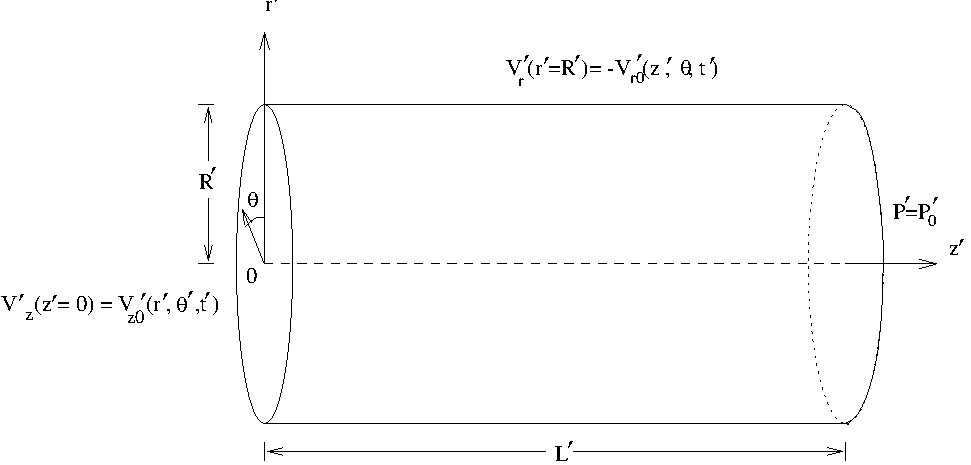
\includegraphics[width=100mm]{figs/cyl.pdf}
    \end{center}
\label{xfigDiagram}
\end{figure}


\begin{figure}[htbp]
    \caption[Bitmap images]{
	The JPEG bitmap format is great for photos but
	crummy for diagrams (including drawings, graphs,
	charts) because it can't gracefully handle sharp edges.
	Note the same bitmap image below from a PNG file and
	from a JPG file; the latter shows characteristic
	``ringing'' at sharp edges -- including text!
	Seriously, magnify and look closely at the JPG's
	awful lines and edges.
	Vector-format PDF is the best for diagrams, but
	if you must use a bitmap image, let it be PNG.
	~ (Left: file {\it drawing.png}.
	Right: file {\it drawing.jpg}.)
	}
    \begin{center}
	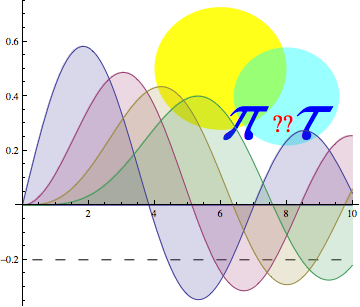
\includegraphics[width=70mm]{figs/drawing.png}
	${}^{}$ ~
	${}^{}$ ~
	${}^{}$
	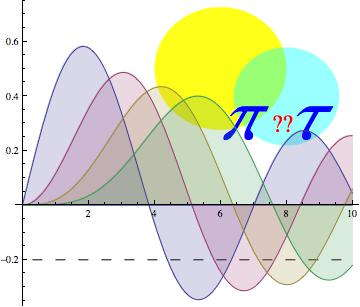
\includegraphics[width=70mm]{figs/drawing.jpg}
    \end{center}
\label{bitmapImages}
\end{figure}



\section{Lists in {\tt thesis} class}

In {\tt thesis} class (for Colorado University),
lists are defined so that nested lists will be
numbered or marked appropriately.
First, an itemized (non-enumerated) list
prefaces each item with a bullet.
Nested itemized list use asterisks,
then dashes, then dots.
These lists are typed between
the \verb2\begin{itemize}2
and \verb2\end{itemize}2
commands.

\begin{itemize}
  \item{} This is ``itemized'' item A.
  \item{} This is ``itemized'' item B.
  \item{} This is ``itemized'' item C.
  \begin{itemize}
    \item{} This is ``itemized'' subitem A.
    \begin{itemize}
      \item{} This is ``itemized'' subsubitem A.
      \begin{itemize}
        \item{} This is ``itemized'' subsubsubitem A.
      \end{itemize}
      \item{} This is ``itemized'' subsubitem B.
    \end{itemize}
    \item{} This is ``itemized'' subitem B.
  \end{itemize}
  \item{} This is ``itemized'' item D.
\end{itemize}

Enumerated lists use the commands
\verb2\begin{enumerate}2 and
\verb2\end{enumerate}2,
and nested enumerations appear like this.

\begin{enumerate}
  \item{} This is ``enumerated'' item A.
  \item{} This is ``enumerated'' item B.
  \item{} This is ``enumerated'' item C.
  \begin{enumerate}
    \item{} This is ``enumerated'' subitem A.
    \begin{enumerate}
      \item{} This is ``enumerated'' subsubitem A.
      \begin{enumerate}
        \item{} This is ``enumerated'' subsubsubitem A.
      \end{enumerate}
      \item{} This is ``enumerated'' subsubitem B.
    \end{enumerate}
    \item{} This is ``enumerated'' subitem B.
  \end{enumerate}
  \item{} This is ``enumerated'' item D.
\end{enumerate}


The work presented
here\footnote{Footnotes are handled neatly by \LaTeX.}
is an extension of Lao\cite{lao:thesis}
and Lao et~al.\cite{lao:paper},
fictional references that are in the bibliographic
source file \verb9refs.bib9.

\begin{table}[htb]
    \caption[Example of a table with its own footnotes]{
	Here is an example of a table with its own footnotes.
	Don't use the $\backslash${\tt footnote} macro if you
	don't want the footnotes at the bottom of the page.
	Also, note that in a thesis the caption goes
	\emph{above} a table, unlike figures.
	}
    \begin{center}
    \begin{tabular}{||l|c|c|c|c||} \hline
	& $S$ & $P$ &   $Q^{\ast}$  & $D^{\dagger}$ \\	% footnote symbols!
	wave form & (kVA) & (kW) & (kVAr) & (kVAd) \\  \hline \hline
	Fig.  \ref{xfigDiagram}a  & 25.48 & 25.00 & -2.82 & 4.03 \\ \hline
	Fig.  \ref{xfigDiagram}b  & 25.11 & 18.02 & -9.75 & 14.52 \\ \hline
	Table \ref{pdftable}  & 24.98 & 22.26 & 9.19 & 6.64 \\ \hline
	Table \ref{powertable}  & 23.48 & 15.00 & 6.59 & 16.82 \\ \hline
	Fig.  \ref{pyramid}  & 24.64 & 22.81 & -0.44 & 9.3 \\ \hline
	\end{tabular}
   \\ \rule{0mm}{5mm}
   ${}^\ast$kVAr means reactive power.		% footnote symbol
\\ ${}^\dagger$kVAd means distortion power.	% footnote symbol
\end{center}
\label{powertable}
\end{table}


